% Options for packages loaded elsewhere
\PassOptionsToPackage{unicode}{hyperref}
\PassOptionsToPackage{hyphens}{url}
%
\documentclass[
  man,LLO-8200, Introduction to Data Science]{apa6}
\usepackage{amsmath,amssymb}
\usepackage{lmodern}
\usepackage{iftex}
\ifPDFTeX
  \usepackage[T1]{fontenc}
  \usepackage[utf8]{inputenc}
  \usepackage{textcomp} % provide euro and other symbols
\else % if luatex or xetex
  \usepackage{unicode-math}
  \defaultfontfeatures{Scale=MatchLowercase}
  \defaultfontfeatures[\rmfamily]{Ligatures=TeX,Scale=1}
\fi
% Use upquote if available, for straight quotes in verbatim environments
\IfFileExists{upquote.sty}{\usepackage{upquote}}{}
\IfFileExists{microtype.sty}{% use microtype if available
  \usepackage[]{microtype}
  \UseMicrotypeSet[protrusion]{basicmath} % disable protrusion for tt fonts
}{}
\makeatletter
\@ifundefined{KOMAClassName}{% if non-KOMA class
  \IfFileExists{parskip.sty}{%
    \usepackage{parskip}
  }{% else
    \setlength{\parindent}{0pt}
    \setlength{\parskip}{6pt plus 2pt minus 1pt}}
}{% if KOMA class
  \KOMAoptions{parskip=half}}
\makeatother
\usepackage{xcolor}
\IfFileExists{xurl.sty}{\usepackage{xurl}}{} % add URL line breaks if available
\IfFileExists{bookmark.sty}{\usepackage{bookmark}}{\usepackage{hyperref}}
\hypersetup{
  pdftitle={Final Report},
  pdfauthor={Bridger Moreland1},
  pdflang={en-EN},
  pdfkeywords={Cyber Bullying},
  hidelinks,
  pdfcreator={LaTeX via pandoc}}
\urlstyle{same} % disable monospaced font for URLs
\usepackage{color}
\usepackage{fancyvrb}
\newcommand{\VerbBar}{|}
\newcommand{\VERB}{\Verb[commandchars=\\\{\}]}
\DefineVerbatimEnvironment{Highlighting}{Verbatim}{commandchars=\\\{\}}
% Add ',fontsize=\small' for more characters per line
\usepackage{framed}
\definecolor{shadecolor}{RGB}{248,248,248}
\newenvironment{Shaded}{\begin{snugshade}}{\end{snugshade}}
\newcommand{\AlertTok}[1]{\textcolor[rgb]{0.94,0.16,0.16}{#1}}
\newcommand{\AnnotationTok}[1]{\textcolor[rgb]{0.56,0.35,0.01}{\textbf{\textit{#1}}}}
\newcommand{\AttributeTok}[1]{\textcolor[rgb]{0.77,0.63,0.00}{#1}}
\newcommand{\BaseNTok}[1]{\textcolor[rgb]{0.00,0.00,0.81}{#1}}
\newcommand{\BuiltInTok}[1]{#1}
\newcommand{\CharTok}[1]{\textcolor[rgb]{0.31,0.60,0.02}{#1}}
\newcommand{\CommentTok}[1]{\textcolor[rgb]{0.56,0.35,0.01}{\textit{#1}}}
\newcommand{\CommentVarTok}[1]{\textcolor[rgb]{0.56,0.35,0.01}{\textbf{\textit{#1}}}}
\newcommand{\ConstantTok}[1]{\textcolor[rgb]{0.00,0.00,0.00}{#1}}
\newcommand{\ControlFlowTok}[1]{\textcolor[rgb]{0.13,0.29,0.53}{\textbf{#1}}}
\newcommand{\DataTypeTok}[1]{\textcolor[rgb]{0.13,0.29,0.53}{#1}}
\newcommand{\DecValTok}[1]{\textcolor[rgb]{0.00,0.00,0.81}{#1}}
\newcommand{\DocumentationTok}[1]{\textcolor[rgb]{0.56,0.35,0.01}{\textbf{\textit{#1}}}}
\newcommand{\ErrorTok}[1]{\textcolor[rgb]{0.64,0.00,0.00}{\textbf{#1}}}
\newcommand{\ExtensionTok}[1]{#1}
\newcommand{\FloatTok}[1]{\textcolor[rgb]{0.00,0.00,0.81}{#1}}
\newcommand{\FunctionTok}[1]{\textcolor[rgb]{0.00,0.00,0.00}{#1}}
\newcommand{\ImportTok}[1]{#1}
\newcommand{\InformationTok}[1]{\textcolor[rgb]{0.56,0.35,0.01}{\textbf{\textit{#1}}}}
\newcommand{\KeywordTok}[1]{\textcolor[rgb]{0.13,0.29,0.53}{\textbf{#1}}}
\newcommand{\NormalTok}[1]{#1}
\newcommand{\OperatorTok}[1]{\textcolor[rgb]{0.81,0.36,0.00}{\textbf{#1}}}
\newcommand{\OtherTok}[1]{\textcolor[rgb]{0.56,0.35,0.01}{#1}}
\newcommand{\PreprocessorTok}[1]{\textcolor[rgb]{0.56,0.35,0.01}{\textit{#1}}}
\newcommand{\RegionMarkerTok}[1]{#1}
\newcommand{\SpecialCharTok}[1]{\textcolor[rgb]{0.00,0.00,0.00}{#1}}
\newcommand{\SpecialStringTok}[1]{\textcolor[rgb]{0.31,0.60,0.02}{#1}}
\newcommand{\StringTok}[1]{\textcolor[rgb]{0.31,0.60,0.02}{#1}}
\newcommand{\VariableTok}[1]{\textcolor[rgb]{0.00,0.00,0.00}{#1}}
\newcommand{\VerbatimStringTok}[1]{\textcolor[rgb]{0.31,0.60,0.02}{#1}}
\newcommand{\WarningTok}[1]{\textcolor[rgb]{0.56,0.35,0.01}{\textbf{\textit{#1}}}}
\usepackage{graphicx}
\makeatletter
\def\maxwidth{\ifdim\Gin@nat@width>\linewidth\linewidth\else\Gin@nat@width\fi}
\def\maxheight{\ifdim\Gin@nat@height>\textheight\textheight\else\Gin@nat@height\fi}
\makeatother
% Scale images if necessary, so that they will not overflow the page
% margins by default, and it is still possible to overwrite the defaults
% using explicit options in \includegraphics[width, height, ...]{}
\setkeys{Gin}{width=\maxwidth,height=\maxheight,keepaspectratio}
% Set default figure placement to htbp
\makeatletter
\def\fps@figure{htbp}
\makeatother
\setlength{\emergencystretch}{3em} % prevent overfull lines
\providecommand{\tightlist}{%
  \setlength{\itemsep}{0pt}\setlength{\parskip}{0pt}}
\setcounter{secnumdepth}{-\maxdimen} % remove section numbering
% Make \paragraph and \subparagraph free-standing
\ifx\paragraph\undefined\else
  \let\oldparagraph\paragraph
  \renewcommand{\paragraph}[1]{\oldparagraph{#1}\mbox{}}
\fi
\ifx\subparagraph\undefined\else
  \let\oldsubparagraph\subparagraph
  \renewcommand{\subparagraph}[1]{\oldsubparagraph{#1}\mbox{}}
\fi
\newlength{\cslhangindent}
\setlength{\cslhangindent}{1.5em}
\newlength{\csllabelwidth}
\setlength{\csllabelwidth}{3em}
\newlength{\cslentryspacingunit} % times entry-spacing
\setlength{\cslentryspacingunit}{\parskip}
\newenvironment{CSLReferences}[2] % #1 hanging-ident, #2 entry spacing
 {% don't indent paragraphs
  \setlength{\parindent}{0pt}
  % turn on hanging indent if param 1 is 1
  \ifodd #1
  \let\oldpar\par
  \def\par{\hangindent=\cslhangindent\oldpar}
  \fi
  % set entry spacing
  \setlength{\parskip}{#2\cslentryspacingunit}
 }%
 {}
\usepackage{calc}
\newcommand{\CSLBlock}[1]{#1\hfill\break}
\newcommand{\CSLLeftMargin}[1]{\parbox[t]{\csllabelwidth}{#1}}
\newcommand{\CSLRightInline}[1]{\parbox[t]{\linewidth - \csllabelwidth}{#1}\break}
\newcommand{\CSLIndent}[1]{\hspace{\cslhangindent}#1}
\ifLuaTeX
\usepackage[bidi=basic]{babel}
\else
\usepackage[bidi=default]{babel}
\fi
\babelprovide[main,import]{english}
% get rid of language-specific shorthands (see #6817):
\let\LanguageShortHands\languageshorthands
\def\languageshorthands#1{}
% Manuscript styling
\usepackage{upgreek}
\captionsetup{font=singlespacing,justification=justified}

% Table formatting
\usepackage{longtable}
\usepackage{lscape}
% \usepackage[counterclockwise]{rotating}   % Landscape page setup for large tables
\usepackage{multirow}		% Table styling
\usepackage{tabularx}		% Control Column width
\usepackage[flushleft]{threeparttable}	% Allows for three part tables with a specified notes section
\usepackage{threeparttablex}            % Lets threeparttable work with longtable

% Create new environments so endfloat can handle them
% \newenvironment{ltable}
%   {\begin{landscape}\centering\begin{threeparttable}}
%   {\end{threeparttable}\end{landscape}}
\newenvironment{lltable}{\begin{landscape}\centering\begin{ThreePartTable}}{\end{ThreePartTable}\end{landscape}}

% Enables adjusting longtable caption width to table width
% Solution found at http://golatex.de/longtable-mit-caption-so-breit-wie-die-tabelle-t15767.html
\makeatletter
\newcommand\LastLTentrywidth{1em}
\newlength\longtablewidth
\setlength{\longtablewidth}{1in}
\newcommand{\getlongtablewidth}{\begingroup \ifcsname LT@\roman{LT@tables}\endcsname \global\longtablewidth=0pt \renewcommand{\LT@entry}[2]{\global\advance\longtablewidth by ##2\relax\gdef\LastLTentrywidth{##2}}\@nameuse{LT@\roman{LT@tables}} \fi \endgroup}

% \setlength{\parindent}{0.5in}
% \setlength{\parskip}{0pt plus 0pt minus 0pt}

% Overwrite redefinition of paragraph and subparagraph by the default LaTeX template
% See https://github.com/crsh/papaja/issues/292
\makeatletter
\renewcommand{\paragraph}{\@startsection{paragraph}{4}{\parindent}%
  {0\baselineskip \@plus 0.2ex \@minus 0.2ex}%
  {-1em}%
  {\normalfont\normalsize\bfseries\itshape\typesectitle}}

\renewcommand{\subparagraph}[1]{\@startsection{subparagraph}{5}{1em}%
  {0\baselineskip \@plus 0.2ex \@minus 0.2ex}%
  {-\z@\relax}%
  {\normalfont\normalsize\itshape\hspace{\parindent}{#1}\textit{\addperi}}{\relax}}
\makeatother

% \usepackage{etoolbox}
\makeatletter
\patchcmd{\HyOrg@maketitle}
  {\section{\normalfont\normalsize\abstractname}}
  {\section*{\normalfont\normalsize\abstractname}}
  {}{\typeout{Failed to patch abstract.}}
\patchcmd{\HyOrg@maketitle}
  {\section{\protect\normalfont{\@title}}}
  {\section*{\protect\normalfont{\@title}}}
  {}{\typeout{Failed to patch title.}}
\makeatother

\usepackage{xpatch}
\makeatletter
\xapptocmd\appendix
  {\xapptocmd\section
    {\addcontentsline{toc}{section}{\appendixname\ifoneappendix\else~\theappendix\fi\\: #1}}
    {}{\InnerPatchFailed}%
  }
{}{\PatchFailed}
\keywords{Cyber Bullying\newline\indent Word count: 1380}
\DeclareDelayedFloatFlavor{ThreePartTable}{table}
\DeclareDelayedFloatFlavor{lltable}{table}
\DeclareDelayedFloatFlavor*{longtable}{table}
\makeatletter
\renewcommand{\efloat@iwrite}[1]{\immediate\expandafter\protected@write\csname efloat@post#1\endcsname{}}
\makeatother
\usepackage{csquotes}
\ifLuaTeX
  \usepackage{selnolig}  % disable illegal ligatures
\fi

\title{Final Report}
\author{Bridger Moreland\textsuperscript{1}}
\date{4/13/2022}


\shorttitle{Final}

\affiliation{\vspace{0.5cm}\textsuperscript{1} Vanderbilt University, Peabody College}

\begin{document}
\maketitle

\hypertarget{research-question}{%
\section{Research Question}\label{research-question}}

With the US holding one of the top spots in Social Network penetration at over 70 percent of the population({``Topic,''} 2022), our country's engagement in social media accounts is consuming increasingly more of our waking time. Along with the proliferation of connected devices and continuous saturation of high-speed internet access comes a reduction in time spent with genuine personal connections and trading face to face experiences for virtual ones, averaging 10\% of our waking time. 70\% of parents estimate that their children spend over four hours per day in virtual interactions on their devices. ({``Cyberbullying,''} 2022) The results of our technology driven obsessions has been a deterioration in empathetic behaviors and other social skills necessary for successfully working within communities, professional teams, and establishing a sense of belonging to groups of people in our lives. Taking the place of friendly banter has been aggression, hostility, and a lack of remorse for how negative actions affect others.

According to Pew Research Center (Auxier, Anderson, Perrin, \& Turner, 2020), four in ten Americans have battled online abuse in some form, often escalating to more severe behaviors such as stalking and sexual harassment. Difficulties arise in quantitative measurements for identifying bullying behaviors and collecting data on their frequencies in given populations as there is no set definition of ``Cyber Bullying''. Researchers must rely on self-reported data from respondents, each with their own list of words and actions they perceive as an attack. Research has begun on identifying factors that influence harassment such as socioeconomic, ethnic, or other diversity criteria. ({``Cyberbullying Research Brief - Archive.ncpc.org,''} 2022) In that vein, I will attempt to assess the pressure points that increase the likely hood of becoming an online victim. My research question for this data analysis will be ``Do household economic indicators (independent variable) indicate an increased likelihood of cyber bullying (dependent variable) in the US?''

\hypertarget{literature-review}{%
\section{Literature Review}\label{literature-review}}

The digital divide doesn't only span generations within the US. There are also obstacles between families with and without access to technology as revealed by studies showing 15\% of students in America do not have access to more than one device at home. (Moore, Vitale, \& Stawinoga, 2018) Aside from a lack of access to devices, those that reside in rural areas face challenges with the ability to access the internet. Astoundingly, nearly three million Americans live in what is considered higher education deserts, meaning they reside 25 miles or more from a public university and lack access to high-speed internet. These differences only amplify the chasm that can be felt between socioeconomic groups within our school system.

The US has moved from the participatory child of previous generations to the one observed by many, and observing many, from the safety of their screens. Under that purview we struggle to protect children from the power of the internet and its ability to disparage and demean the people on the other side of mindless messaging. Of those that will speak up against it, forty-three percent of teens reported being victims of cyberbullying in the past year. ({``Cyberbullying Research Brief - Archive.ncpc.org,''} 2022) It has become a force to manage within the daily demands of educators and employers alike, distracting from learning and workplace productivity. The ease at which perpetrators can attack without leaving their couch has fast become one of the laziest crimes in America, with the added destructive result of emotional and physical toil on its victims.
The rise of social media, and the technology impact in general, adds to the general feeling that children are being exposed at too young an age to dogma that they are not yet equipped to process. One of the more popular platforms with children under 11, YouTube, does more than entertain that age group. About 46\% of parents reported that their child was exposed to videos that were age inappropriate for them. (Auxier et al., 2020) In the attempt to shield the younger generation from these ills, surveyed parents across demographics consider it harder to raise children in today's age of technology. Limited screen time seems to be one of the bigger challenges in controlling a child's environment as percent of time per day devoted to technology continues to rise in the younger generation. The technology struggle, however, isn't limited to children, as 68\% of parents also admit to being distracted by their devices when they are spending time with their children.

The combination of an always on, always connected, mentality along with the disassociation with physical groups only worsens the impact of the disturbing trend in cyber bulling among the US population. While all types of bullying have been prevalent in our past, that same affliction to force ones will on another through feelings of jealousy, fear, distrust, and the overall need dominate through mental or verbal abuse, has been magnified through the lens of a connected world. What once was pain that could be hidden is now blasted to the masses and documented for posterity, taunting the prey and impeding recovery from the victimization. And the attacks are escalating. Severe forms of harassment, physical threats, sexual harassment, and stalking, only made up 15\% of incidents reported in 2014 and has now grown to 25\% of today's cyber bullying incidents. (Auxier et al., 2020)

Due to the reverse impact socioeconomic standing has on internet and device availability, it is believed that the more affluent social media users will be victimized to a greater extend by Cyber Bullies than those from lesser household means. The following data is presented as a review of how a family's income could possibly increase chances of falling victim to personal cyber-attacks through social media.

\hypertarget{data-analysis}{%
\section{Data analysis}\label{data-analysis}}

For this effort I will be using a data set derived from the US Census Bureau where respondents were asked about online harassment, stalking, or cyber-bullying for any member of their household. Only three of their most current supplemental surveys address these specific data elements. Data was collected from the July, 2015, November, 2017, and November 2019 versions of the Current Population Survey, Computer, and Internet Use Supplement ({``Current Population Survey, November 2019 ... - Census.gov,''} 2019).

\hypertarget{census-dataset-summary}{%
\subsection{Census Dataset Summary}\label{census-dataset-summary}}

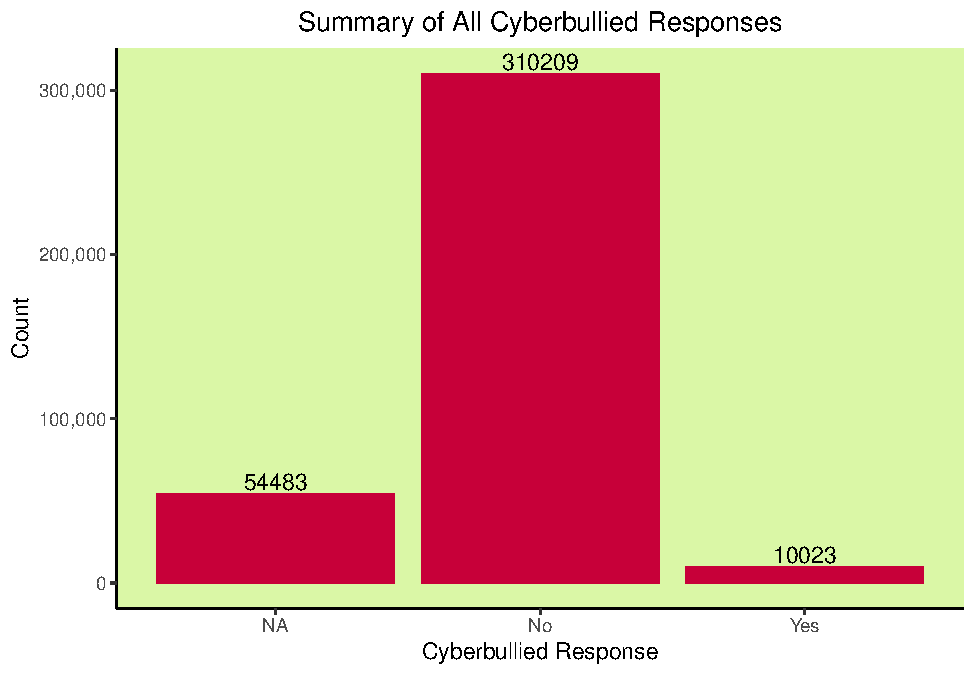
\includegraphics{CyberBully_files/figure-latex/SummarizeCyberbullyResponses-1.pdf}

\hypertarget{cyberbullying-experienced-in-the-us-by-household-income-levels.}{%
\subsection{Cyberbullying Experienced in the US by Household Income Levels.}\label{cyberbullying-experienced-in-the-us-by-household-income-levels.}}

\begin{Shaded}
\begin{Highlighting}[]
\NormalTok{knitr}\SpecialCharTok{::}\NormalTok{opts\_chunk}\SpecialCharTok{$}\FunctionTok{set}\NormalTok{(}\AttributeTok{echo =} \ConstantTok{FALSE}\NormalTok{, }\AttributeTok{warning =} \ConstantTok{FALSE}\NormalTok{, }\AttributeTok{message =} \ConstantTok{FALSE}\NormalTok{)}

\NormalTok{Income\_Bullied }\OtherTok{\textless{}{-}}\NormalTok{ dfCPSComputerSupplement }\SpecialCharTok{\%\textgreater{}\%} \FunctionTok{count}\NormalTok{(FamilyIncome, FamilyIncomeRange, CyberBulliedAnswer, InterviewYear)}
\NormalTok{Income\_Bullied }\OtherTok{\textless{}{-}} \FunctionTok{filter}\NormalTok{(Income\_Bullied, CyberBulliedAnswer}\SpecialCharTok{==}\StringTok{"Yes"}\NormalTok{)}
\NormalTok{Income\_Bullied}\SpecialCharTok{$}\NormalTok{Sqrt.n }\OtherTok{\textless{}{-}} \FunctionTok{sqrt}\NormalTok{(Income\_Bullied}\SpecialCharTok{$}\NormalTok{n)}
\CommentTok{\# Income\_Bullied[order(as.numeric(Income\_Bullied$FamilyIncome)),]}

\CommentTok{\# Build Histogram}
\NormalTok{Income\_Bullied.heatmap }\OtherTok{\textless{}{-}}\NormalTok{ Income\_Bullied }\SpecialCharTok{\%\textgreater{}\%}
  \FunctionTok{ggplot}\NormalTok{(}\AttributeTok{data =}\NormalTok{ Income\_Bullied,}
         \AttributeTok{mapping =} \FunctionTok{aes}\NormalTok{(}
           \AttributeTok{x =}\NormalTok{ InterviewYear,}
           \AttributeTok{y =} \FunctionTok{reorder}\NormalTok{(FamilyIncomeRange, }\FunctionTok{as.integer}\NormalTok{(FamilyIncome)),}
           \AttributeTok{fill =}\NormalTok{ Sqrt.n}
\NormalTok{         )) }\SpecialCharTok{+}
  \FunctionTok{geom\_tile}\NormalTok{() }\SpecialCharTok{+}
  \FunctionTok{xlab}\NormalTok{(}\AttributeTok{label =} \StringTok{"Reported Occurences of Cyberbullying"}\NormalTok{) }\SpecialCharTok{+}
  \FunctionTok{ylab}\NormalTok{(}\AttributeTok{label =} \StringTok{"Family Income Bracket"}\NormalTok{) }\SpecialCharTok{+}
  \FunctionTok{ggtitle}\NormalTok{(}\AttributeTok{label =} \StringTok{"Cyberbullying Experienced in the US by Household Income Levels"}\NormalTok{) }\SpecialCharTok{+}
  \FunctionTok{facet\_grid}\NormalTok{( }\SpecialCharTok{\textasciitilde{}}\NormalTok{ InterviewYear, }\AttributeTok{scales =} \StringTok{"free\_x"}\NormalTok{, }\AttributeTok{space =} \StringTok{"free\_x"}\NormalTok{) }\SpecialCharTok{+}
  \FunctionTok{theme}\NormalTok{(}
    \AttributeTok{axis.text.x =} \FunctionTok{element\_blank}\NormalTok{(),}
    \AttributeTok{axis.ticks.x =} \FunctionTok{element\_blank}\NormalTok{(),}
    \AttributeTok{plot.title =} \FunctionTok{element\_text}\NormalTok{(}\AttributeTok{hjust =} \FloatTok{0.5}\NormalTok{),}
    \AttributeTok{strip.background =} \FunctionTok{element\_rect}\NormalTok{(}\AttributeTok{fill =} \StringTok{"\#EEEEEE"}\NormalTok{, }\AttributeTok{color =} \StringTok{"\#EEEEEE"}\NormalTok{)}
\NormalTok{  ) }\SpecialCharTok{+}
  \FunctionTok{scale\_fill\_gradient}\NormalTok{(}\AttributeTok{name =} \StringTok{"Sqrt(n)"}\NormalTok{,}
                      \AttributeTok{low =}\NormalTok{ themecolor1,}
                      \AttributeTok{high =}\NormalTok{ themecolor2)}

\NormalTok{Income\_Bullied.heatmap}
\end{Highlighting}
\end{Shaded}

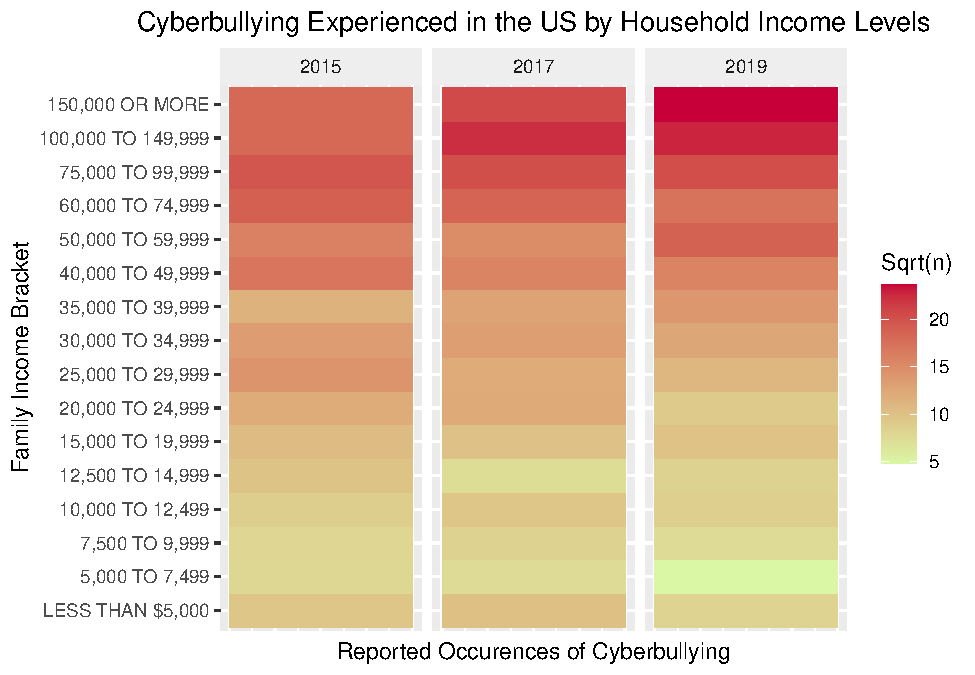
\includegraphics{CyberBully_files/figure-latex/CyberbullyByIncome-1.pdf}
\#\# Cyberbullying Occurances by Gender

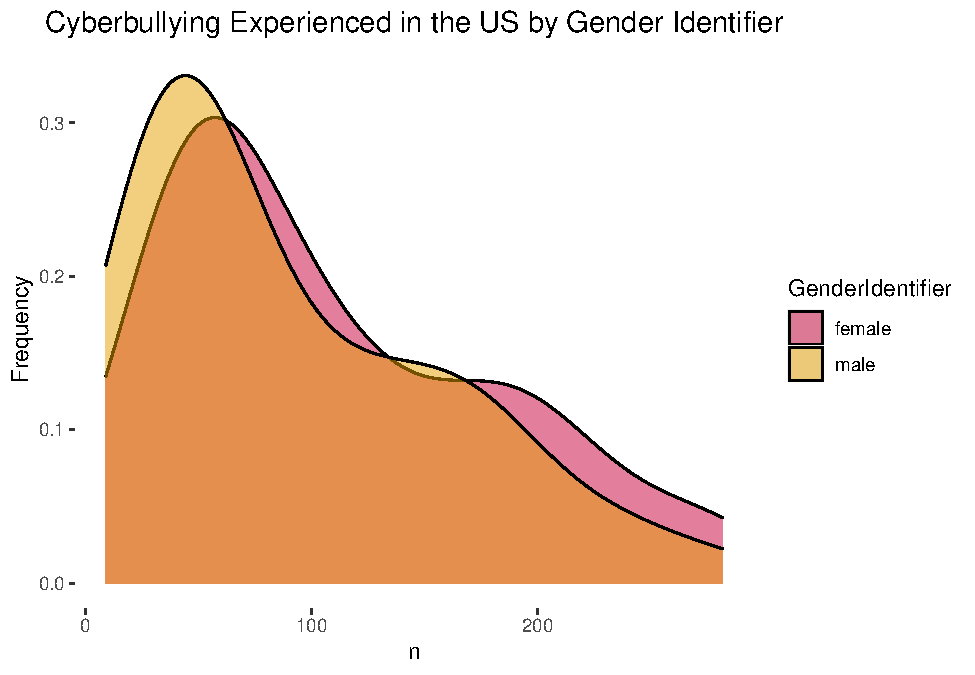
\includegraphics{CyberBully_files/figure-latex/unnamed-chunk-1-1.pdf} 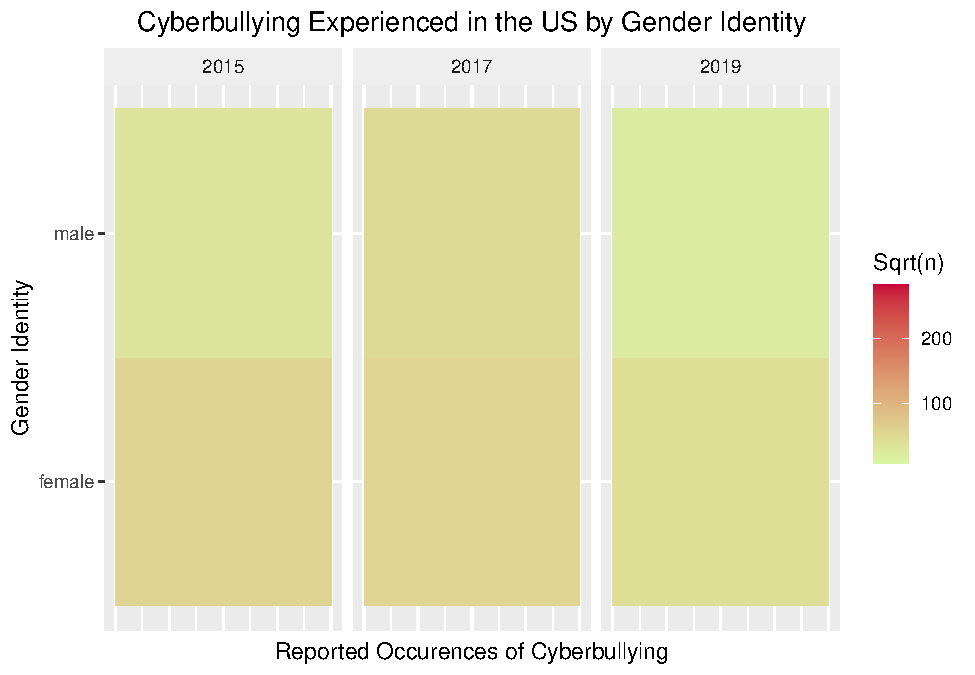
\includegraphics{CyberBully_files/figure-latex/unnamed-chunk-1-2.pdf}

\hypertarget{cyber-bullying-experienced-in-the-us-by-state.}{%
\subsection{Cyber Bullying experienced in the US by State.}\label{cyber-bullying-experienced-in-the-us-by-state.}}

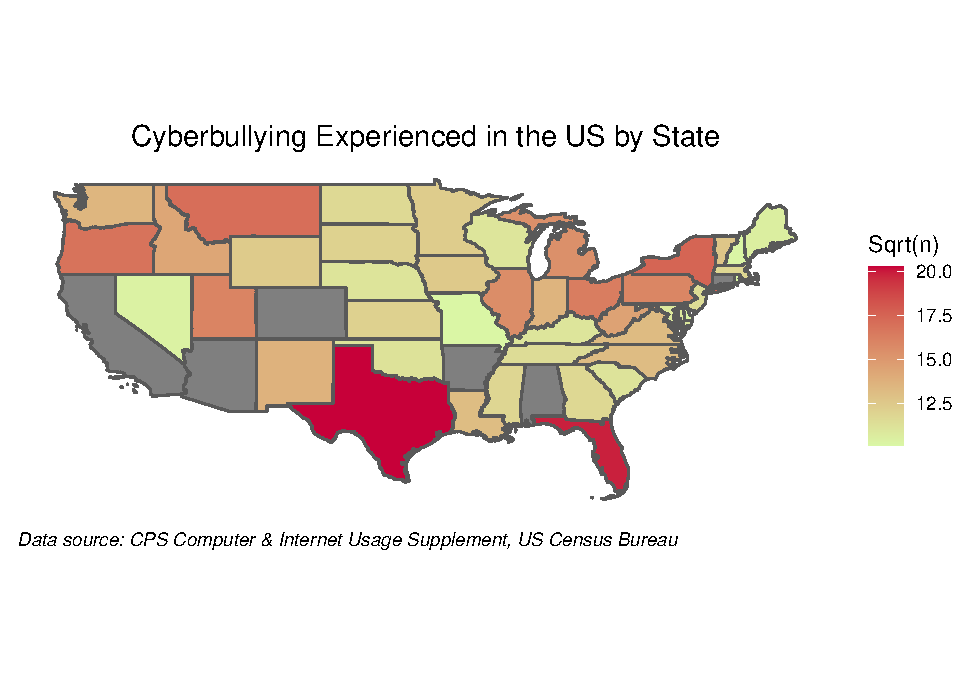
\includegraphics{CyberBully_files/figure-latex/CyberbullyByState-1.pdf}

\hypertarget{cyberbullying-occurences-by-age}{%
\subsection{Cyberbullying Occurences by Age}\label{cyberbullying-occurences-by-age}}

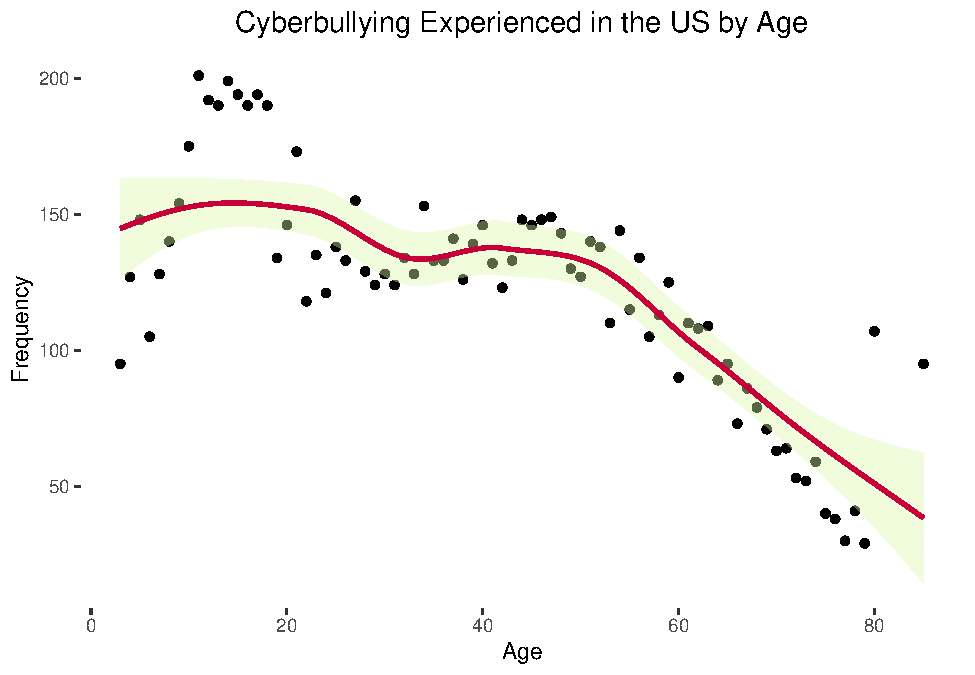
\includegraphics{CyberBully_files/figure-latex/DemographicIndicators-1.pdf}

\hypertarget{conditional-mean-of-dependent-variables}{%
\subsection{Conditional mean of dependent variables:}\label{conditional-mean-of-dependent-variables}}

\hypertarget{bivariate-graphics-comparing-dependent-variables-with-independent-variables}{%
\subsection{Bivariate graphics comparing dependent variables with independent variables:}\label{bivariate-graphics-comparing-dependent-variables-with-independent-variables}}

\hypertarget{next-steps}{%
\section{Next Steps}\label{next-steps}}

The next steps toward identifying possible leading indicators of targets to Cyber Bullying will include extending the temporal data set with a second census survey and analyzing any changes in reported Cyber Bullying cases using data science tools available in R, a validation of the predictive model, and a summary of the findings.

\newpage

\hypertarget{references}{%
\section*{References}\label{references}}
\addcontentsline{toc}{section}{References}

\hypertarget{refs}{}
\begin{CSLReferences}{1}{0}
\leavevmode\vadjust pre{\hypertarget{ref-auxier_anderson_perrin_turner_2020}{}}%
Auxier, B., Anderson, M., Perrin, A., \& Turner, E. (2020). Parenting children in the age of screens. Pew Research Center. Retrieved from \url{https://www.pewresearch.org/internet/2020/07/28/parenting-children-in-the-age-of-screens/}

\leavevmode\vadjust pre{\hypertarget{ref-2019_cps_computer_and_internet_use_2019}{}}%
Current population survey, november 2019 ... - census.gov. (2019). United States Census Bureau. Retrieved from \url{https://www2.census.gov/programs-surveys/cps/techdocs/cpsnov19.pdf}

\leavevmode\vadjust pre{\hypertarget{ref-national_crime_prevention_council_2022}{}}%
Cyberbullying research brief - archive.ncpc.org. (2022). Retrieved from \url{http://archive.ncpc.org/resources/files/pdf/bullying/Cyberbullying\%20research\%20brief.pdf}

\leavevmode\vadjust pre{\hypertarget{ref-security_2022}{}}%
Cyberbullying: Twenty crucial statistics for 2022. (2022). Security.org. Retrieved from \url{https://www.security.org/resources/cyberbullying-facts-statistics/}

\leavevmode\vadjust pre{\hypertarget{ref-e;_2020}{}}%
E;, L.-M. E.-C. E.-Z. M.-S. (2020). Socioeconomic effects in cyberbullying: Global research trends in the educational context. U.S. National Library of Medicine. Retrieved from \url{https://pubmed.ncbi.nlm.nih.gov/32570762/}

\leavevmode\vadjust pre{\hypertarget{ref-moore_vitale_stawinoga_2018}{}}%
Moore, R., Vitale, D., \& Stawinoga, N. (2018). The digital divide and educational equity. Retrieved from \url{https://www.act.org/content/dam/act/unsecured/documents/R1698-digital-divide-2018-08.pdf?ref=hackernoon.com}

\leavevmode\vadjust pre{\hypertarget{ref-statista_2022}{}}%
Topic: Social media usage in the united states. (2022). Statista Research Department. Retrieved from \url{https://www.statista.com/topics/3196/social-media-usage-in-the-united-states/\#topicHeader__wrapper}

\end{CSLReferences}


\end{document}
